\section{Symmetric Cryptography}
Block Ciphers: map blocks of symbols of fixed length $n$ into blocks of the same length.\\
\begin{tabular}{|l l |l|}
	\hline
	Vigenère Cipher &	encryption	&	$E_z: \mathbb{Z}_m^n \to \mathbb{Z}_m^n, \mathbf{v} \mapsto \mathbf{v} + \mathbf{z} \mod m$ \\
							         \cline{2-3}
	(16th century) & decryption & $D_z: \mathbb{Z}_m^n \to \mathbb{Z}_m^n, \mathbf{v} \mapsto \mathbf{v} - \mathbf{z} \mod m$ \\
	\hline
	Hill Cipher & encryption & $E_M: \mathbb{Z}_m^n \to \mathbb{Z}_m^n, \mathbf{v} \mapsto M\mathbf{v} \mod m$ \\
							         \cline{2-3}
	(1929) & decryption & $D_M: \mathbb{Z}_m^n \to \mathbb{Z}_m^n, \mathbf{v} \mapsto M^{-1}\mathbf{v} \mod m$ \\
	& & $M$ is an $(n \times n)$-matrix with elements in $\mathbb{Z}_m$ \\
	\hline
	General & encryption & $E_{(M,\mathbf{b})}: \mathbb{Z}_m^n \to \mathbb{Z}_m^n, \mathbf{v} \mapsto M\mathbf{v} + \mathbf{b} \mod m$ \\
							         \cline{2-3}
	affine linear cipher & decryption & $D_{(M,\mathbf{b})}: \mathbb{Z}_m^n \to \mathbb{Z}_m^n, \mathbf{v} \mapsto M^{-1}\mathbf{v} - \mathbf{b} \mod m$ \\
	\hline
\end{tabular}

\subsubsection{Cryptanalysis of historical block ciphers}
\begin{tabular}{|cccccccccccccccccccccccccc|} %{llllllllllllllllllllllllll}
	\hline
	a & b & c & d & e & f & g & h & i & j & k  & l  & m  & n  & o  & p  & q  & r  & s  & t  & u  & v  & w  & x  & y  & z  \\
	0 & 1 & 2 & 3 & 4 & 5 & 6 & 7 & 8 & 9 & 10 & 11 & 12 & 13 & 14 & 15 & 16 & 17 & 18 & 19 & 20 & 21 & 22 & 23 & 24 & 25 \\
	\hline
\end{tabular}\\
Modulus $m=26$\\

Need: $n+1$ plaintexts $\bm w_i$ and the corresponding ciphertexts $\mathbf{c}_i= M\mathbf{w}_i+ \mathbf{b} \mod m$.\\
$W=(\bm w_1-\bm w_0, \ldots , \bm w_n-\bm w_0)  \mod m$ and $C=(\bm c_1-\bm c_0, \ldots , \bm c_n-\bm c_0) \mod m$ \\
$\Rightarrow \text{if } gcd(det(W),m)=1 \text{ then } M=CW^{-1} \mod m$ and $\bm b=\bm c_0-M\bm w_0 \mod m$.\\
For Hill cipher we set $\bm w_0=\bm c_0 = \bm 0 \Rightarrow \bm b=0$; For Vigen\'{e}re cipher we set the $M = I$\\
Without knowledge of the plaintext, the plaintext can be estimated with the known statistics of a language. 

\subsubsection{Secure Block Ciphers}
The plaintexts $X$ and ciphertexts $Y$ are bit strings of length $n$ and the keys $K$ are bit strings of length $r$. Then a cryptographic algorithm $E$ defines equations that hold for each ciphertext bit:\\
\begin{minipage}{0.25\linewidth}
$y_1 = F_1(x_1,\ldots,x_n,k_1,\ldots,k_r)$\\
$\ldots = \ldots$\\
$y_n = F_n(x_1,\ldots,x_n,k_1,\ldots,k_r)$
\end{minipage}
\begin{minipage}{0.35\linewidth}
\textbf{Confusion:}
\begin{liste}
	\item $F_i$ should be mathematically complex
	\item For a given $\mathbf{x}$ and $\mathbf{y}$, it is not feasible to solve for $\mathbf{k}$
	\item $F_i$ must not be linear
\end{liste}
\end{minipage}
\begin{minipage}{0.35\linewidth}
\textbf{Diffusion:}
\begin{liste}
	\item Changing a single bit in the plaintext (or the key), on average $50\%$ of the ciphertext bits should change
	\item ''Every ciphertext bit should depend on every plaintext and every key bit''
\end{liste}
\end{minipage}

To achieve confusion and diffusion, many block ciphers are product ciphers: $E = E_R \circ E_{R-1} \circ \ldots \circ E_2 \circ E_1$ where $E_i$ are round functions and each uses a round key that is derived from the secret key (key scheduling) and $R$ is the number of rounds.
Nonlinearity is achieved using S-boxes: $S: \mathbb{Z}_2^m \rightarrow \mathbb{Z}_2^n$.
Security is achieved by sufficiently many rounds!

\subsubsection{Modes of Operation of Block Ciphers}%TODO: continue
Notation: $IV$ = Initial Vector, $P_i$ = Plaintext, $C_i$ = Cipher, $E_k(x)$ = encryption function with key $k$, $D_k(x)$ = decryption function with key $k$\\
\begin{tabular}{|l l |p{12cm}|}
\hline
	ECB	&	Electronic Code Book Mode	&	plaintext divided into $n$-bit blocks. Each block encryped by $E$ individually. \\
		&								&	Drawback: same plaintext goes into same cipher $\to$ gives information about the plaintext or the order of the ciphertext can be changed.\\
\hline
	CBC	&	Cipher Block Chaining Mode	&	enc: $C_1=E_k(P_1 \oplus IV), \quad C_i=E_k(P_i \oplus C_{i-1})$ \\
		&								&	dec: $P_1=D_k(C_1) \oplus IV, \quad P_i=D_k(C_i) \oplus C_{i-1}$	\\	
\hline
	CFB &	Cipher Feedback Mode		& 	enc: $C_1=P_1 \oplus E_k(IV), \quad C_i=P_i \oplus E_k(C_{i-1})$\\
		&								&	dec: $P_1=C_1 \oplus E_k(IV), \quad P_i=C_i \oplus E_k(C_{i-1})$\\
		&								&	Drawback: error propagation. Benefit: selfsync.\\
\hline
	OFB	&	Output Feedback Mode		& 	enc: $C_1=\underbrace{E_k(IV)}_{\tilde{C_1}} \oplus P_1, \quad C_i=\underbrace{E_k(\tilde{C}_{i-1})}_{\tilde{C_i}} \oplus P_i $\\
		&								& 	dec: $P_1=E_k(IV) \oplus C_1, \quad P_i=E_k(C_{i-1}) \oplus C_i $\\
		&								&	Drawback: not self synchronizing. Each message needs a different IV.\\
\hline
	CTR	&	Counter Mode				& 	enc: $C_i=P_i \oplus E_k(ctr_i) $, $ctr_i$: counter reading.\\
		&								&	dec: $P_i=C_i \oplus E_k(ctr_i) $\\
		&               & Drawback: each counter value only once $\rightarrow$ Nonce. Benefit: enc/dec parallel, no error propagation.\\
\hline
\end{tabular}\\

Period: $\approx 2^{\frac{n}{2}} \to $ birthday paradox. After about $2^{\frac{n}{2}}$ encryptions, the output of the block cipher repeats.

\subsection{DES (Data Encryption Standard)}
\begin{minipage}{10cm}
\begin{liste}
\item 16 Rounds with 56bit (thank you NSA) key each. 64bits of plaintext are ciphered. Nonlinearity comes from S-Boxes.
\item IP $=$ Initial Permutation, FP $=$ Final Permutation
\item One Round looks like: $T(L,R)=(L \oplus F_k(R),R)$ and $M(L,R)=(R,L)$
\item Transformations are involutions $\to$ two times the same operation gives the initial value.
\item $C=IP^{-1} \circ T_{16} \circ M \circ T_{15} \circ \ldots \circ M \circ T_1 \circ IP(P)$
\item $P=IP^{-1} \circ T_1 \circ  M \circ T_2 \circ \ldots \circ M \circ T_{16} \circ IP(C)$
\end{liste}
The $F$-Function works as follows:
\begin{liste}
\item The input (32-bit) is extended to 48-bit with some bits copied. Additionally the bits are permuted. ($E$-Box)
\item The data is now XOR-added with the 48-bit round key and put into 8 S-boxes.
\item The S-boxes have a nonlinear function and map the 8 different 6-bit input to 4-bit. ($S$-Boxes)
\item The output bits are permuted again. ($P$-Boxes)
\end{liste}
The big disadvantage is, that the DES algorithm just uses a 56bit key.\\
To avoid this disadvantage the Double DES was developed with the drawback of meet-in-the-middle attack. It works like this:
\begin{aufzaehlung}
    \item For every possible $DES$ key $k_i$, compute $M_i = DES(C,k_i)$ and store the tuple $(M_i, k_i)$.\\
    \item Loop again through all possible $DES$ keys $k_j$ and compute $N_j = DES^{-1}(C,k-j)$. Check whether $N_j$ 
    is the same as one of your stored $M_i$. If you find a match, it's pretty likely that you've just 
    found the two keys you're looking for!\\
    (1. table with $2^{56}$ 64bit keys, 2. table with $2^{56}$ 64bit keys $\to$ $2^{112-64} = 2^{48}$ analogies.)\\
\end{aufzaehlung}
Notes:
\begin{liste}
	\item DES is very efficient to implement in hardware, but not so in software.
  \item Better solution: Triple DES $\to$ key size = 112-bit or 168-bit.
  \item Better solution: IDEA is very efficient to implement in software, but not so in hardware (128-bit key and multiplications instead of S-Box).
\end{liste}


\subsection{AES (Advanced Encryption Standard)}
Some marketing numbers: 128 bit block size, 128, 192 or 256 bit keys. AES is an iterated block cipher with n number of $N_r$ rounds
with $N_{r_{128}}=10, N_{r_{192}}=12, N_{r_{256}}=14$. Drawback: encryption differs from decryption.\\
One round of AES consist of three layers:\\
- Nonlinear Layer: 16 parallel 8$\times$8-bit S-boxes with optimal nonlinearity.\\
- Linear Mixing Layer: Effects good diffusion.\\
- Key Additon Layer: Usual XOR of the round key with the actual internal state.\\

\end{minipage}
\hspace{5mm}
\begin{minipage}{7cm}
\begin{center}
  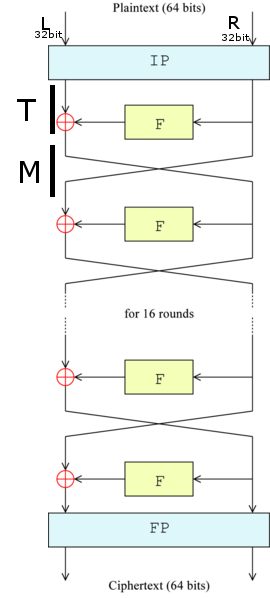
\includegraphics[width=5.5cm]{./bilder/DES-main-network.png}\\
  Schemata of the \em DES main network \em\\
  \vspace{2mm}
  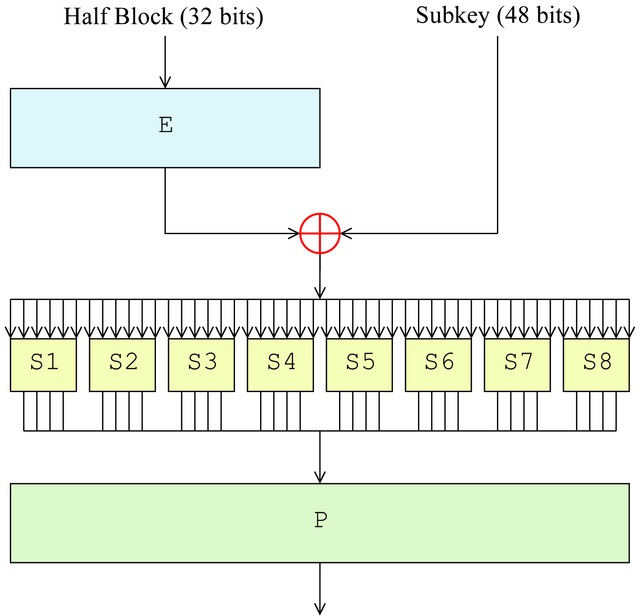
\includegraphics[width=7cm]{./bilder/DES-f-function.png}\\
  Schemata of the DES \em F\em-Function\\
 \end{center}
\end{minipage}

\begin{multicols}{2}
Encryption-pseudocode:
\begin{verbatim}
Store input bits into state matrix
AddRoundKey
while (Count rounds from 1 to NumberOfRounds-1) {
  SubBytes
  ShiftRows
  MixColumns
  AddRoundKey
}
SubBytes
ShiftRows
AddRoundKey
Return state matrix
\end{verbatim}

\textbf{AddRoundKey:}
XOR each column of the state matrix with the corresponding word from the round key.

\textbf{SubBytes:}
Take the multiplicative inverse in GF($2^8$) (map $\{00\}$ to $\{00\}$), then: affine Transformation over GF($2^8$).

\textbf{ShiftRows:}
Bytes in the last three rows of the state are cyclically shifted over different number of byte.

\textbf{MixColumns:}
Columns are considered as polynomials over GF($2^8$) and multiplied modulo $x^4+1$ with a fixed polynomial: $a(x) = \{03\} \cdot x^3 + \{01\} \cdot x^2 + \{01\} \cdot x + \{02\}$
\end{multicols}

\subsection{IDEA (International Data Encryption Algorithm)}
\begin{multicols}{2}
\begin{liste}
	\item 128-bit key
	\item Confusion: Mixes three ''incompatible'' group operations so that no two successive operations are of the same type.
	\item Diffusion: Provided for by the ''Multiply-Add (M-A) Box''.
	\item Encryption/Decryption similarity: Differ only in the key schedule used.
	\item Scalable: Mini-versions (2,4,8-bit symbols) can be used for analysis.
	\item Transparency: No ''random-looking'' tables or ''mysterious'' S-boxes.
	\item Easy to substitute for DES: Both have 64-bit plain-/ciphertexts
\end{liste}

Operations:
\begin{liste}
	\item [\-] $\oplus$ Bit-by-bit modulo-two addition (XOR)
	\item [\-] $\boxplus$ Addition modulo $2^{16}$
	\item [\-] $\odot$ Multiplication modulo $2^{16} + 1$ of nonzero numbers
\end{liste}
The output of one operation never goes to another operation of the same kind $\rightarrow$ Confusion.

\begin{minipage}{0.5\linewidth}
Multiply-Add Box:\\
Provides Diffusion. This is the simplest structure with this property!
\end{minipage}
\begin{minipage}{0.5\linewidth}
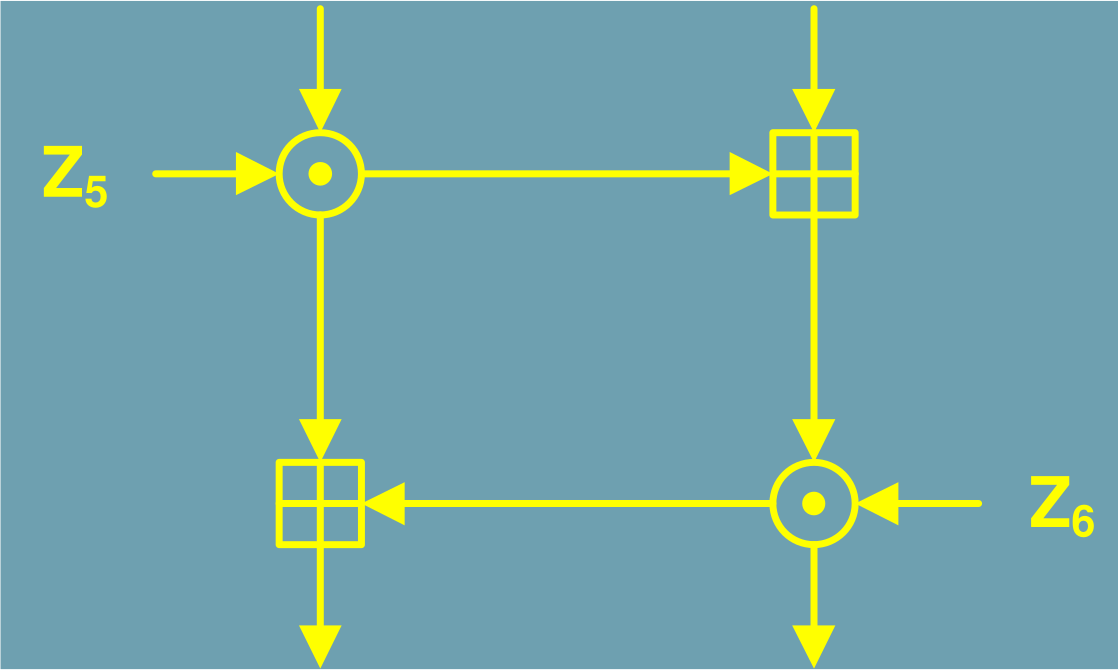
\includegraphics[width=0.8\linewidth]{./bilder/MultiplyAdd.png}
\end{minipage}

\vfill\null
\columnbreak
\begin{minipage}{\linewidth}
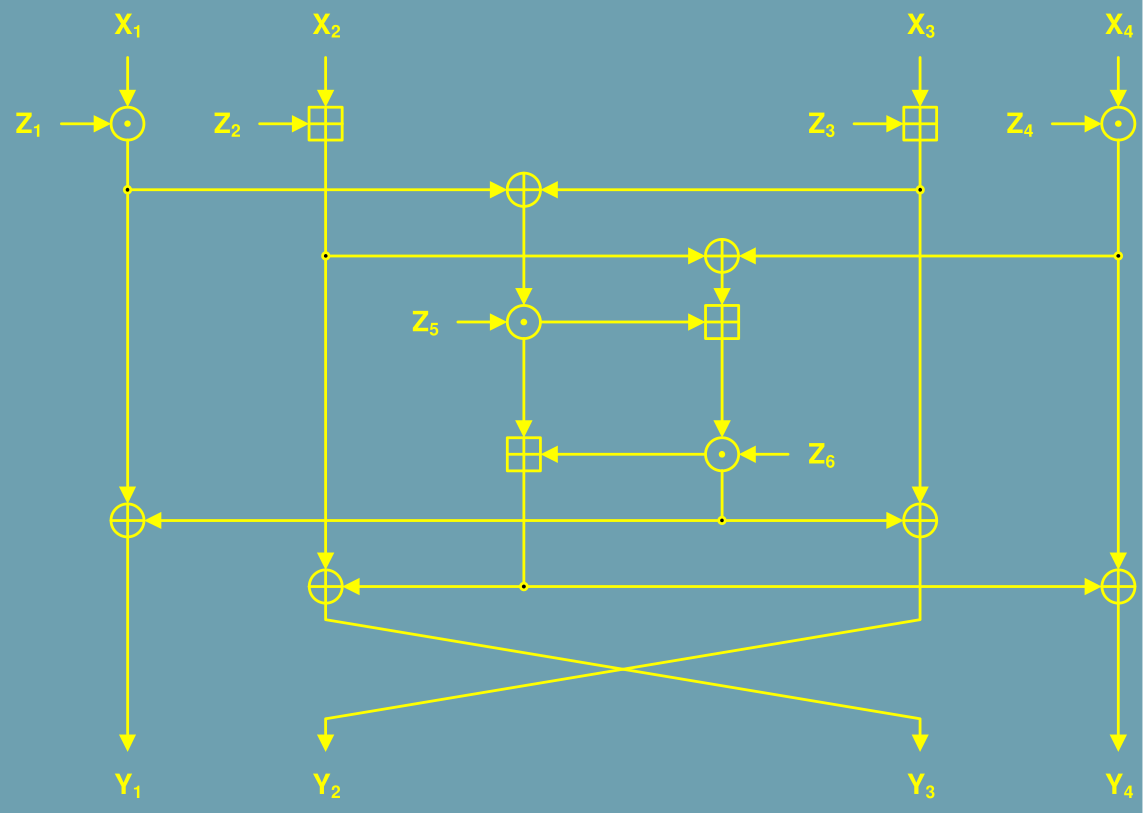
\includegraphics[width=0.8\linewidth]{./bilder/IDEA_structure.png}\\
An IDEA encryption round, $Z_1, \ldots, Z_6$: Round keys (16 bits)\\
\end{minipage}

Final round:\\
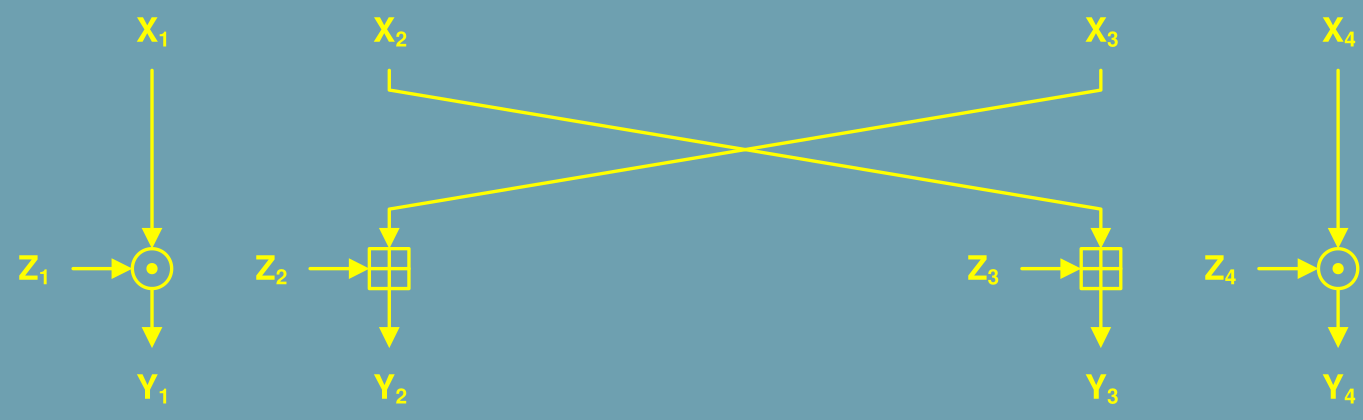
\includegraphics[width=\linewidth]{./bilder/IDEA_final_round.png}
Causes that the same structure can be used to encrypt and decrypt (just use the inverses of the round keys in reverse order).
\end{multicols}

\subsection{PGP (Pretty Good Privacy)}
PGP uses block ciphers and is used for file encryption on a computer, computation of private and public RSA keys, and for sending and receiving of encrypted emails.\\
PGP is a set of different methods.\\
Necessary steps:
\begin{aufzaehlung}
\item A session key is generated.
\item The message is encrypted with a block cipher unsing the session key (IDEA and other block ciphers).
\item RSA is used to encrypt the session key with the public key of the receiver.
\item The encrypted message and the encrypted session key are bundled to a message that is mailed to the receiver.\\
\end{aufzaehlung}
PGP works without public key infrastructure (web of trust is used).

\subsubsection{Conclusion}
\begin{liste}
\item AES fast, RSA (based on Diffie-Hellmann) slow
\item AES need previous knowledge 
\item RSA for key-exchange, and AES/IDEA/DES for message cipher.
\end{liste}
